\section{Ejercicio 7}
En este experimento observaremos el error cuadrático medio para cada estimador en función de $n$, con $n$ siendo la cantidad de muestras de tamaño $15$. En el gráfico siguiente, podemos observar que errores cuadráticos medios de cada estimador convergen a valores no nulos. En particular, observando los datos adquiridos en el \textbf{ejercicio 4}, podemos observar que el error cuadrático medio de $\hat{\theta}_{mv}$, $\hat{\theta}_{mom}$ y $\hat{\theta}_{med}$ tienden a $0.003$, $0.022$ y $0.057$ respectivamente, que no coincidentalmente aproximan al valor de sus varianzas con $n \rightarrow \infty$. ¿Esto significa que los estimadores son insesgados? Probablemente. Lo analizaremos adelante.

\begin{figure}[H]
	\centering
	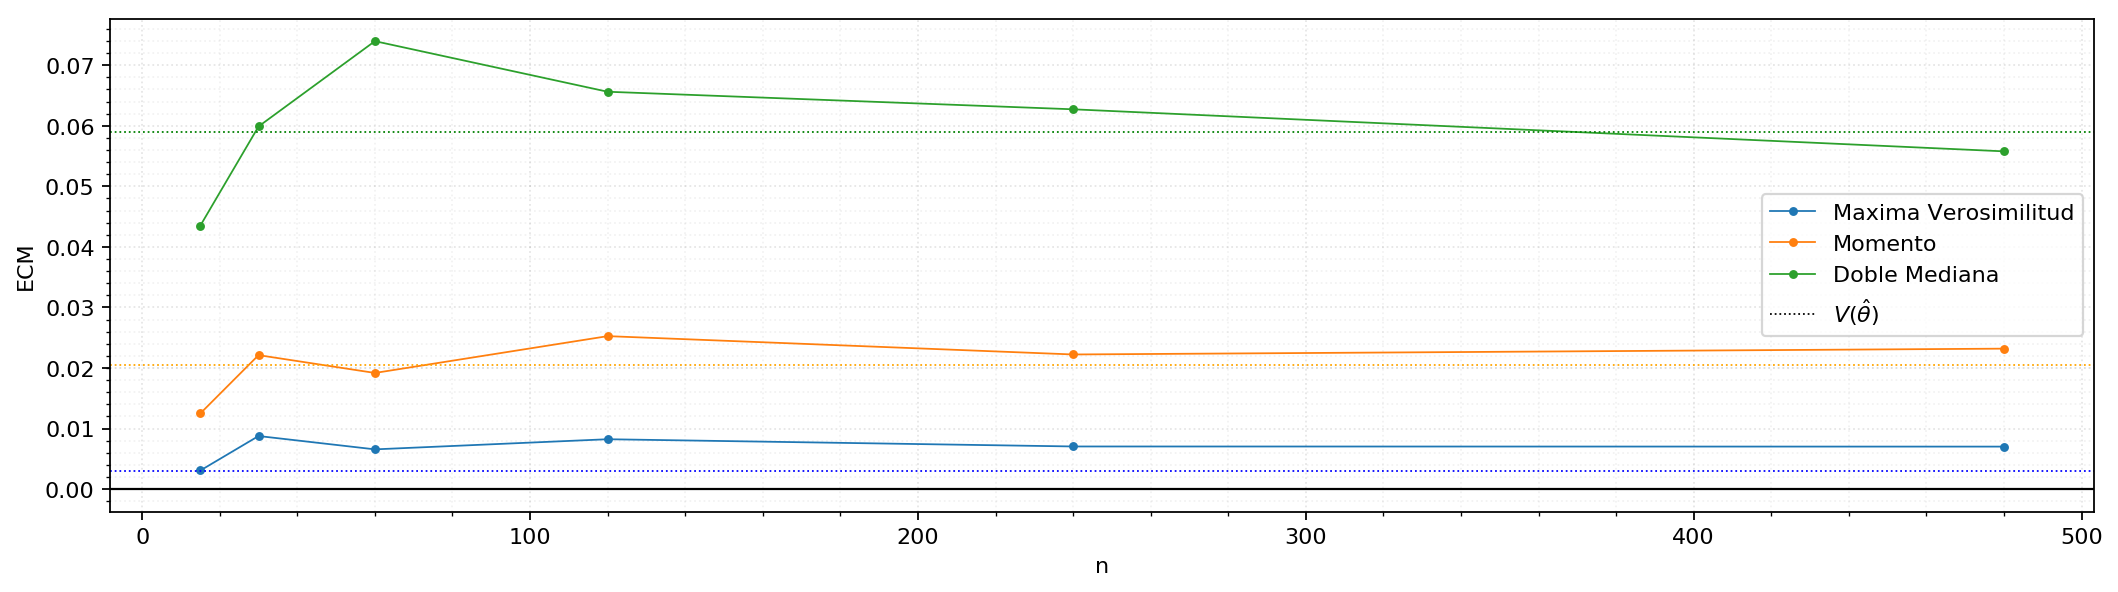
\includegraphics[width=1\textwidth]{imagenes/ecm-en-f-de-n.png}
	\caption{\footnotesize ECM de los estimadores en función de n. $a=0, b=1$}
	\label{fig:ej7-ecm-en-f-de-n}
\end{figure}

Observando el gráfico \ref{fig:ej7-ecm-en-f-de-n}, podemos sospechar que los errores cuadráticos medios de los tres estimadores tienden a la varianza cuando $n$ es muy grande. Podemos hipotetizar que los estimadores son consistentes, sobretodo porque en la figura \ref{fig:ej7-sesgos-en-f-de-n} se aprecia que el sesgo de los estimadores tiende a cero a medida que $n$ crece, es decir, los estimadores son – por lo menos – asintoticamente insesgados. Veamos los sesgos de los estimadores a medida que $n \rightarrow \infty$:

\begin{figure}[H]
	\centering
	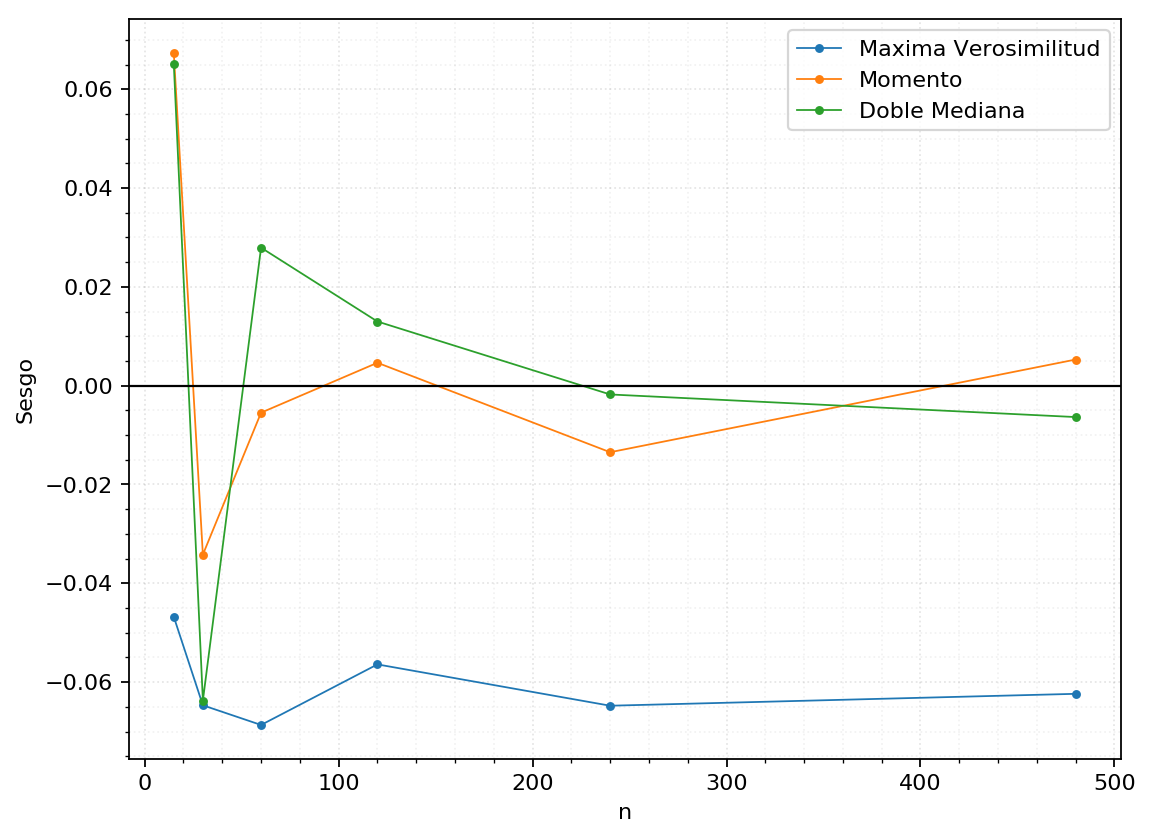
\includegraphics[width=1\textwidth]{imagenes/sesgos-en-f-de-n.png}
	\caption{\footnotesize Sesgos de los estimadores en función de n. $a=0, b=1$}
	\label{fig:ej7-sesgos-en-f-de-n}
\end{figure}

Podemos conjeturar, entonces, que los sesgos de los estimadores $\hat{\theta}_{mom}$ y $\hat{\theta}_{med}$ tienden a cero. ¿Pero qué hay del estimador de máxima verosimilitud? Si calculamos $E(\hat{\theta}_{mv})$, llegaremos a que equivale a $\frac{n}{n+1} * \theta$, que si bien no es igual a $\theta$, sí tiende a este valor cuando $n \rightarrow \infty$. Luego el estimador de máxima verosimilitud es asintóticamente insesgado por lo tanto los errores cuadráticos medios de los estimadores efectivamente tienden a sus varianzas, y estas varianzas son muy cercanas a cero. Finalmente, como los estimadores son asintóticamente insesgados y sus varianzas se asimilan al valor nulo, se puede sospechar que son consistentes.

\begin{figure}[H]
	\centering
	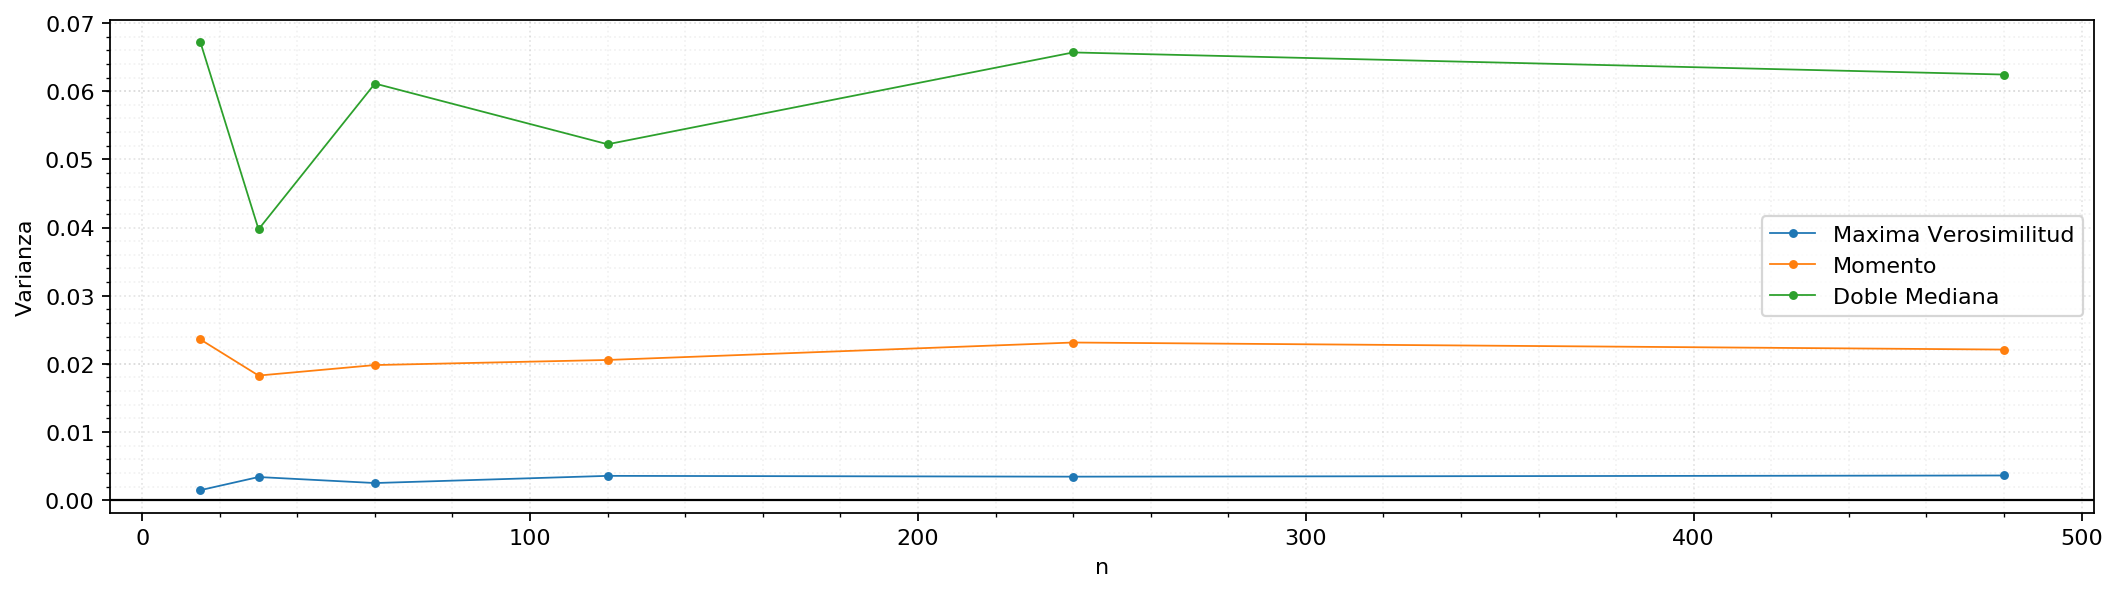
\includegraphics[width=1\textwidth]{imagenes/varianzas-en-f-de-n-small.png}
	\caption{\footnotesize Varianzas de los estimadores en función de n. $a=0, b=1$}
	\label{fig:ej7-varianzas-en-f-de-n-small}
\end{figure}